[134~v\textsuperscript{o}] employant assez toute la force de l'air elle ne peut pas soustenir quelque chose d'avantage; ainsi il faut que l'eau entre \textit{B} et \textit{CD} soit entierement soûtenue par la force unitive, sans que l'air du Recipient \textit{EE} y contribue la moindre chose. Cela pos\'{e}, il s'ensuit, que pendant que la bulle d'air monte entre \textit{A} et \textit{B} il n'arrive pas plus de changement, que s'il n'y avoit point du tout de bulle, ou si \edtext{l'eau}{\lemma{si}\Afootnote{ \textit{ (1) }\ la bulle \textit{ (2) }\  l'eau \textit{ L}}} \edtext{\textit{AB} estoit soûten\"{u}e d'un fond, ou si elle n'estoit pas purg\'{e}e}{\lemma{\textit{AB}}\Afootnote{ \textit{ (1) }\ n'estoit point purg\'{e}e, ou si elle \textit{ (2) }\ estoit [...] purg\'{e}e \textit{ L}}}, \`{a} cause que la force unitive, laquelle seule peut estre chang\'{e}e par la bulle d'air, n'y contribue rien. Mais sitost que la bulle d'air entre dans la region de cette eau qui est soûten\"{u}e par la force unitive du mouuement general: alors il y a trois efforts l'un du mouuement general \`{a} dilater la bulle (car c'est l\`{a} \edtext{où il faut chercher l'explication du ressort de l'air}{\lemma{l\`{a}}\Afootnote{ \textit{ (1) }\ par où il faut expliquer le ressort de l'air \textit{ (2) }\ où [...] l'air \textit{ L}}}) l'autre du mouuement general \`{a} empecher la desunion des corps\protect\index{Sachverzeichnis}{corps}\edtext{}{\lemma{}\Afootnote{corps  \textbar\ sensibles \textit{ gestr.}\ \textbar\ (car \textit{ L}}} \edtext{(car c'est l\`{a} où il faut chercher l'explication de l'attachement dans le vuide\protect\index{Sachverzeichnis}{vide})}{\lemma{}\Afootnote{(car c'est l\`{a}  \textit{ (1) }\ par où il faut expliquer l'attachement \textit{ (2) }\ où [...] vuide\protect\index{Sachverzeichnis}{vide}) \textit{ erg.} \textit{ L}}}, la troisi\`{e}me  du mouuement general \`{a} pousser les corps\protect\index{Sachverzeichnis}{corps} grossiers (comme l'eau) vers le centre du globe, (car c'est l\`{a} \edtext{où il faut chercher la raison de}{\lemma{l\`{a}}\Afootnote{ \textit{ (1) }\ par où il faut expliquer \textit{ (2) }\ où [...] de \textit{ L}}} la pesanteur) l'effort \edtext{deuxieme}{\lemma{}\Afootnote{deuxieme \textit{ erg.} \textit{ L}}} de la force unitive et \edtext{le troisi\`{e}me}{\lemma{}\Afootnote{le troisi\`{e}me \textit{ erg.} \textit{ L}}} de la pesanteur \edtext{se combattoient}{\lemma{pesanteur}\Afootnote{ \textit{ (1) }\ combattoient ensemble, sans conciliation \textit{ (2) }\ se combattoient \textit{ L}}}; \edtext{mais la bulle estant arriv\'{e}e, [phenomene 8.]\edtext{}{\Afootnote{8\textit{\ L \"{a}ndert Hrsg.}}} avec l'effort, qu'elle a de se dilater qui est le premier, elle nous donne le moyen de les concilier}{\lemma{mais}\Afootnote{ \textit{ (1) }\ il se  \textit{(a)}\ trouue \textit{(b)}\ rencontre un moyen de les concilier, ou de trouuer le milieu, par l'arriv\'{e}e de la bulle \textit{ (2) }\ la [...] dilater \textit{(a)}\ , car auparavant \textit{(b)}\ qui [...] concilier \textit{ L}}}. Car le deuxieme \edtext{(de la force unitive)}{\lemma{}\Afootnote{(de la force unitive) \textit{ erg.} \textit{ L}}} tache d'empecher la desunion des corps sensibles\protect\index{Sachverzeichnis}{corps!sensible}, le troisiesme \edtext{(de la pesanteur)}{\lemma{}\Afootnote{(de la pesanteur) \textit{ erg.} \textit{ L}}} tache \edtext{d'effectuer}{\lemma{tache}\Afootnote{ \textit{ (1) }\ de procurer \textit{ (2) }\ d'effectuer \textit{ L}}} la desunion de l'eau et du verre, et par consequent pendant qu'il n'y a point de corps sensibles\protect\index{Sachverzeichnis}{corps!sensible}, que l'eau et le verre, ils se combattront; mais sitost que le troisiesme (du ressort de la bulle) \edtext{vient \`{a} s'exercer}{\lemma{bulle)}\Afootnote{ \textit{ (1) }\ arrive \textit{ (2) }\ vient \`{a} s'exercer \textit{ L}}}, alors il se trouue un moyen d'empecher la desunion des corps sensibles\protect\index{Sachverzeichnis}{corps!sensible}; selon l'effort troisi\`{e}me, sans empecher la desunion de l'eau et du verre contre l'effort deuxieme, parce que la bulle d'air se mettant entre l'eau et le verre, leur desunion se fait sans \edtext{une}{\lemma{}\Afootnote{une \textit{ erg.} \textit{ L}}} desunion des corps\protect\index{Sachverzeichnis}{corps!sensible} sensibles. Et ainsi la bulle d'air estant mont\'{e} jusque \`{a} ce qu'elle touche la superficie interieure du verre en \textit{B} fend en un moment l'union du verre et de l'eau, et s'elle dilate par la superficie interieure de tout le matras, \`{a} cause \edtext{non seulement de son propre effort \`{a} se dilater mais aussi parce que les deux autres}{\lemma{cause}\Afootnote{ \textit{ (1) }\ que les deux \textit{ (2) }\ non [...] autres \textit{ L}}} efforts combattans sont bien ais\'{e}s de luy ouurir par tout le chemin pour \edtext{s'y}{\lemma{}\Afootnote{s'y \textit{ erg.} \textit{ L}}} glisser entre \edtext{deux corps, et pour se concilier ensemble ces deux efforts contraires}{\lemma{entre}\Afootnote{ \textit{ (1) }\ les deux, et pour les concilier ensemble \textit{ (2) }\ deux [...] contraires \textit{ L}}} de sorte que l'effort du ressort de la bulle, et de la pesanteur de la liqueur\protect\index{Sachverzeichnis}{liqueur} obtiennent leur effect, sans que la force unitive en souffre.\selectlanguage{latin}
\pend 
%Zeitz auskommentiert\begin{center}
%                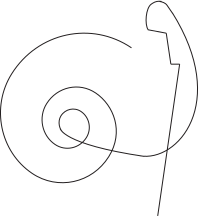
\includegraphics[width=0.5\textwidth]{images/37_3_134r2}\\\textit{[Fig. 3, nicht zuzuordnende Zeichnung]}
%\end{center}